\chapter{物理信息-生成式正逆向流变学本构建模研究}
% 引言 引出第四章内容
\section{引言}
流变学本构建模长期面临实验数据与理论模型间的鸿沟。传统方法常基于理想化假设构建本构方程,虽然可以获得数学模型,却难以准确表征真实材料在复杂工况下的非线性响应。基于前章通过PI-GRU网络对流变数据的时序建模基础,本章则提出物理信息驱动与生成式建模融合的新范式,通过融合频率域的真实实验数据与物理守恒定律的强约束机制,构建兼具高预测精度与可定制性的智能建模框架。

当前流变学本构建模领域存在两大核心问题,第一个问题是传统物理模型在描述真实材料复杂流变行为时,常因过度简化导致预测偏差累积,而纯数据驱动的黑箱模型虽能实现高精度拟合,却丧失了物理可解释性这一流变学研究的本质诉求,同时由于流变学数据往往依赖于各类流变仪的实验测量,所以优质的流变学数据是稀有的,本文前一章使用数值模拟方法可以生成大量模拟数据,但是这在真实实验上不可以复刻。Mahmoudabadbozchelou提出的一类PINN方法,通过多保真建模,首先通过对实验数据进行本构方程的参数拟合,然后借用拟合后的方程进行数值模拟生成大量低保真数据,之后使用高保真数据(原本的实验数据)和低保真数据(模拟数据)联合进行深度学习训练,在一定程度上缓解了数据不足问题,同时由于低保真数据本身是符合经典本构方程的,具有一定物理约束意义。本章参考了Mahmoudabadbozchelou的方法,来对一类黏弹性聚合物凝胶的流变学数据:储存模量($\mathrm{G^{\prime}}$)、损耗模量($\mathrm{G^{\prime\prime}}$)和损耗角正切(tan$\delta$)进行PINN建模,尝试构建材料制备参数、频率到流变学性质的模型映射。在Mahmoudabadbozchelou的基础模型中,本文引入了几个优化,首先是通过引入可学习的损失函数权重,使得模型在训练过程中,能够根据训练数据中不同参数的分布情况,动态调整损失函数的权重,从而提高模型泛化能力,其次在特征工程方面,引入注意力特征融合的方法,进一步解决实验数据特征稀疏的问题。

第二个问题是材料逆向设计过程中,基于试错法的实验优化模式耗费大量资源,而现有生成模型在流变学参数空间的可控生成方面缺乏物理约束,导致生成结果常偏离热力学可行域。近年来,许多研究者聚焦于材料制备参数到流变学性质的建模,但是实际应用中,根据已知的期望的材料性质,通过反向建模来确定这种材料应该如何制备也是非常重要。考虑到多组分材料体系的流变指纹具有高维参数空间中的低维流形特性,VAE的潜空间建模应用于流变学的反向建模是可行的,本章使用了VAE类模型中的CVAE来进行反向建模,探究特定制备参数到流变学特性的可控映射。

本章创新性地将PINN与CVAE进行耦合,建立双向建模通道:在正向建模路径中,通过将已知的本构方程编码为PINN的软约束条件,有效解决了小样本实验数据下的过拟合问题;在逆向设计路径中,利用CVAE的潜空间探索能力,结合流变响应的物理可行性验证模块,实现了从目标流变特性到材料制备参数的可控映射。这种混合建模策略不仅突破了传统方法在数据-物理融合层面的技术壁垒,更重要的是构建了闭环的材料设计-验证工作流,为智能流变学提供一定方法论基础。
% 实验设计  描述本章的实验过程,介绍黄金的工作,模型相关公式等等
\section{实验设计}
\subsection{PINN-CVAE正逆向建模架构} \label{PINN-CVAE架构}
本章构建了PINN-CVAE正逆向建模架构,如图\ref{PINN-CVAE-illustration}所示。
本章首先使用PINN模型对低保真数据和高保真数据进行训练。模型架构包含两个MLP网络:低保真网络$\mathbf{M_{low}}$和高保真网络$\mathbf{M_{high}}$。训练流程如下:

低保真数据$X_{low}$首先通过低保真网络得到预测值$\hat{y}_{low}$,与真实低保真标签$y_{low}$计算物理损失。之后高保真数据$X_{high}$通过低保真网络得到中间特征$f_{mid}$,将$f_{mid}$与$X_{high}$拼接后输入高保真网络,得到最终预测值$\hat{y}_{high}$。$\hat{y}_{high}$与真实高保真标签$y_{high}$计算数据损失,并与物理损失拼接得到总损失。

具体计算过程可表示为公式\eqref{eq:lf-model}和公式\eqref{eq:hf-model}:
\begin{align}
  \hat{y}_{low}  & = \mathbf{M_{low}}(X_{low}) \label{eq:lf-model}                               \\
  \hat{y}_{high} & = \mathbf{M_{high}}(X_{high}, \mathbf{M_{low}}(X_{high})) \label{eq:hf-model}
\end{align}

在损失函数选择上,考虑到实验数据中可能存在的异常值和噪声,本文采用鲁棒性较好的Huber损失函数,其定义如公式\eqref{eq:huber-loss}所示:
\begin{equation}
  \begin{aligned}
    \mathcal{L}_\delta(y, \hat{y}) =
    \begin{cases}
      \frac{1}{2}(y - \hat{y})^2                 & \text{if } |y - \hat{y}| \le \delta    \\
      \delta |y - \hat{y}| - \frac{1}{2}\delta^2 & \text{otherwise} \label{eq:huber-loss}
    \end{cases}
  \end{aligned}
\end{equation}
Huber损失函数通过参数$\delta$实现对异常值敏感度的动态调节:当$\delta$趋近于0时,其行为接近MAE,表现出对异常值的强鲁棒性;当$\delta$较大时,其特性近似于MSE,保持了较高的训练效率。这种自适应特性使得模型能够在保持训练稳定性的同时,有效应对实验数据中的噪声干扰。

本章在基本的PINN损失函数构建公式中添加可学习的权重$\alpha$,如公式\eqref{eq:pinn-loss-weight},通过权重$\alpha$平衡损失强度,适应不同的训练任务。
\begin{equation}
  \mathcal{L}_{\text{PINN}} = \underbrace{\mathcal{L}_\delta(y_{low}, \hat{y}_{low})}_{\text{低保真物理损失}} + \alpha \cdot \underbrace{\mathcal{L}_\delta(y_{high}, \hat{y}_{high})}_{\text{高保真数据损失}}+L_{2}  \label{eq:pinn-loss-weight}
\end{equation}


之后本章使用CVAE进行反向建模,输入特征为[$\omega$、$\mathrm{G^{\prime}}$、$\mathrm{G^{\prime\prime}}$、tan$\delta$]序列,输出标签为制备参数:$M_{n_i}$和$w_i$。CVAE的损失函数公式如公式\eqref{eq:cvae-expriment}所示,其中$x = [w, \mathrm{G^{\prime}}, \mathrm{G^{\prime\prime}}, \tan \delta]$,$p = { M_{n_i}, w_i }'$。
\begin{equation}
  \mathcal{L}(\theta_E, \theta_D) = \mathbb{E}{q{\theta_E}(z|\mathbf{x},p)} \left[ \log p_{\theta_D}(\mathbf{x}|z,p) \right] - D_{KL}\left(q_{\theta_E}(z|\mathbf{x},p) | p(z|p)\right) \label{eq:cvae-expriment}
\end{equation}
\begin{figure}[htbp]
  \centering
  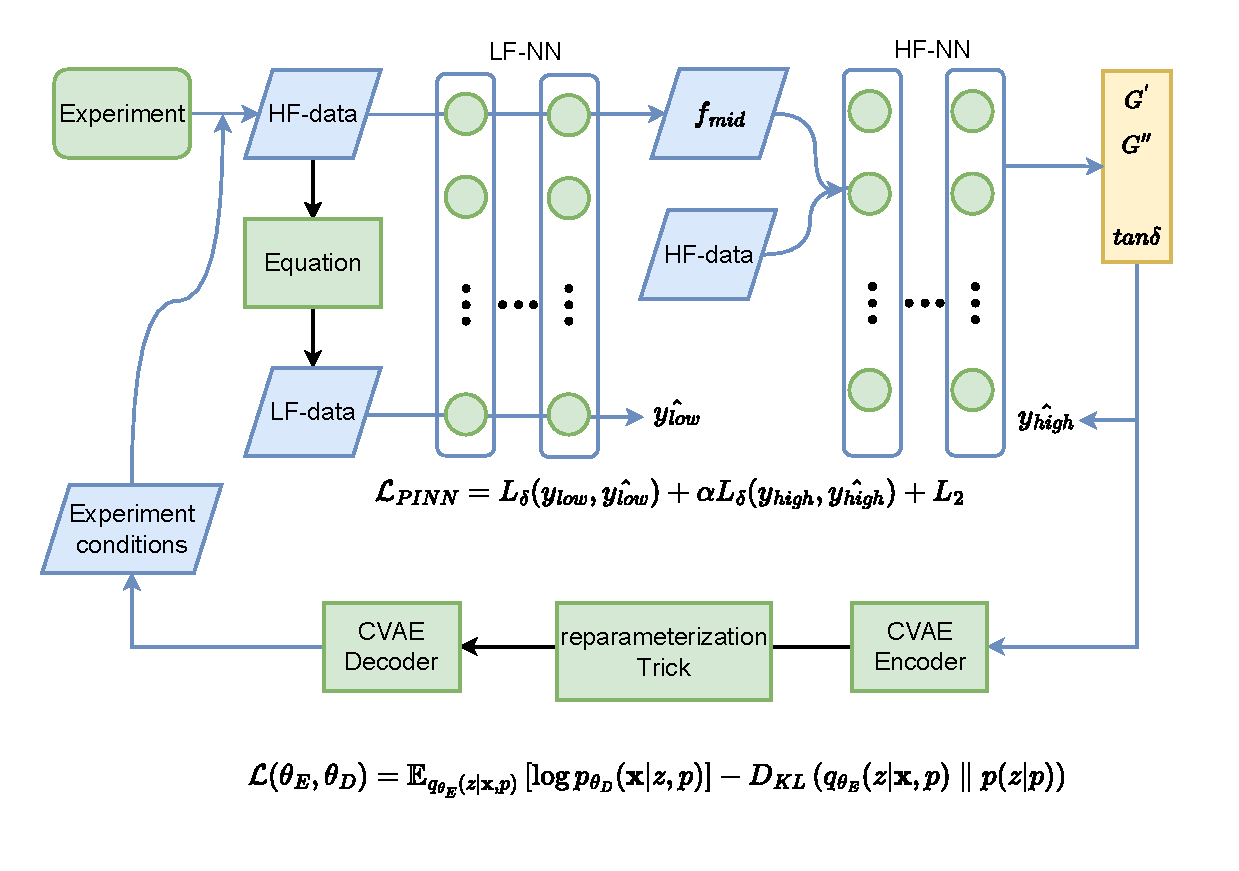
\includegraphics[width=0.8\textwidth]{Fig/PINN-CVAE.pdf}
  \FigureBicaption{\label{PINN-CVAE-illustration}PINN-CVAE正逆向建模架构}{Schematic illustration of the PINN-CVAE model}
\end{figure}

通过建立PINN-CVAE的联合建模,可以建立一个自适应增强的流变学机器学习系统。该系统的工作流程如下:首先,PINN模型通过物理约束和特征融合机制对流变学数据进行正向建模,建立组分特征到流变学性质的映射关系。在实际应用过程中,通过真实实验获得的新数据可以不断补充到训练集中,进一步提升PINN模型的预测精度。与此同时,CVAE模型负责从目标流变学性质反向生成可能的组分配比方案,为材料设计提供多样化的参考。这些由CVAE生成的组分方案可以输入到PINN模型中进行快速评估和筛选,通过比较预测曲线与目标曲线的吻合度,筛选出最具潜力的组分配比进行实验验证,从而大大减轻实验负担。最后,实验验证结果又可以作为新的训练数据反馈给两个模型,形成一个不断优化的闭环系统。这种联合建模方法充分发挥了两种模型的优势,既保证了预测的物理合理性,又提供了材料设计的多样化方案,同时通过数据驱动和实验验证的结合,实现了系统性能的持续提升。

\subsection{数据预处理}
\subsubsection{实验数据来源}
本章所有训练和测试的实验数据是基于Huang等人的工作\cite{huangUltrahighEnergydissipationElastomers2021}。Huang等人介绍了一种黏性的聚丙烯酸正丁酯(Poly(n-butyl acrylate), PBA)流体注入弹性网络中,形成聚合物流体凝胶(Polymer Fluid Gels, PFGs),以实现宽频带可控超高能量耗散的策略,如图\ref{huangjin-illustration}所示。
\begin{figure}[htbp]
  \centering
  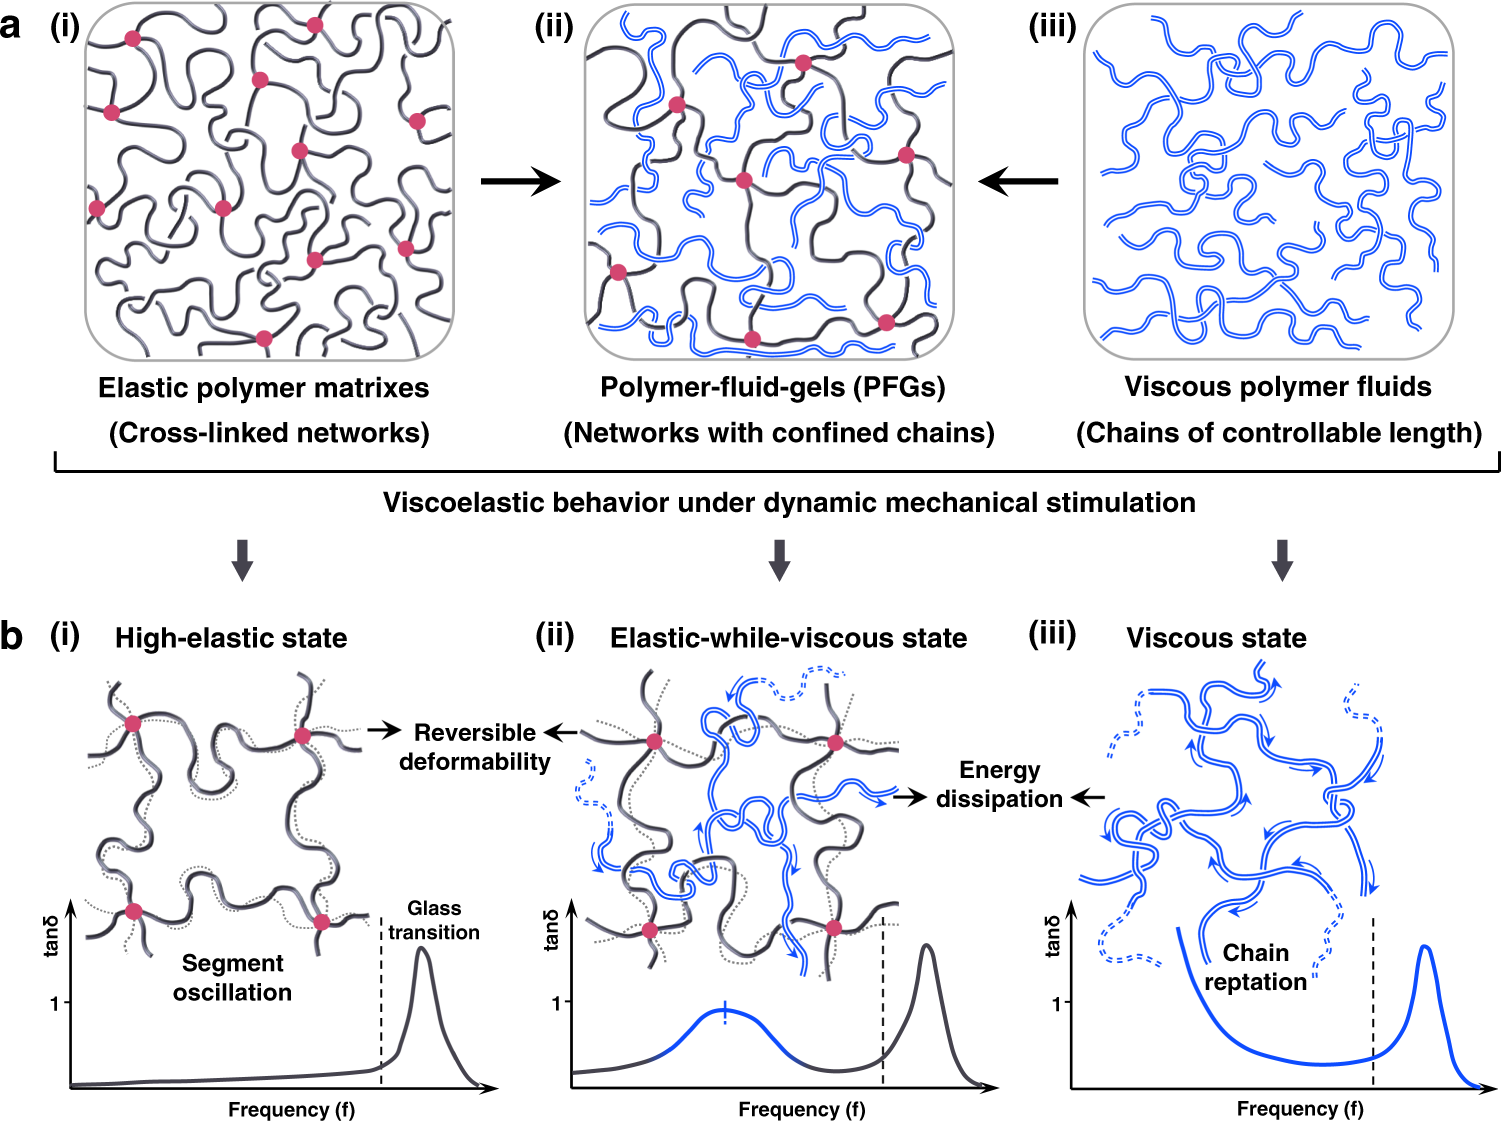
\includegraphics[width=0.8\textwidth]{Fig/huangjin.png}
  \FigureBicaption{\label{huangjin-illustration}Huang等人制备的PFGs示意图\cite{huangUltrahighEnergydissipationElastomers2021}}{Schematic illustration of the PFGs prepared by Huang et al\cite{huangUltrahighEnergydissipationElastomers2021}}
\end{figure}
在实验过程中,Huang等人对不同分子量的PBA流体,注入不同分子量PBA制备的PFGs,分别进行了流变学实验,得到了对应材料特定频率下的储存模量、损耗模量和损耗角正切等数据。本章采用他们的实验数据进行具体的深度学习建模。

\subsubsection{实验数据分类}
首先本章对真实实验数据进行分类,第一类为单PBA流体数据,为不同分子量的PBA流体的流变学数据,特征包括:聚合度(Degree of Polymerization, DP)、数均分子量(Mn)、分散指数(Polymer Dispersity Index, PDI)、频率($\omega$),标签包括:储存模量($\mathrm{G^{\prime}}$)、损耗模量($\mathrm{G^{\prime\prime}}$)和损耗角正切(tan$\delta$),第二类为单分子量PBA注入制备的PFGs数据,特征和标签和第一类单PBA流体数据一致,第三类为多分子量PBA注入制备的PFGs数据,特征包括:不同分子量的PBA特征和组分信息(Mn$_i$、PDI$_i$、DP$_i$、$\phi_i$,$i=1,2,3$)、$\omega$,标签包括:$\mathrm{G^{\prime}}$、$\mathrm{G^{\prime\prime}}$和tan$\delta$。第三类数据的组分信息见表\ref{pba-com-groups}所示。
\begin{table}
  \TableBicaption{\label{pba-com-groups}多分子量PBA流体制备PFGs的配比参数表}{Formulation Parameters of Multi-MW PBA Fluids for PFGs}
  \centering
  \small
  \begin{tabularx}{\textwidth}{>{\centering\arraybackslash}X >{\centering\arraybackslash}X} % 关键修改点
    \Xhline{1.5pt}
    实验分组   & \makecell{
      \begin{tabular}{@{}c@{}}
        $\phi_{PBA}(\%)$ \\
        \Xhline{0.5pt}
        Mn(20k,35k,52k,78k,102k,152k)
      \end{tabular}
    }                         \\
    \Xhline{0.5pt}
    PFG-b1 & (0,20,0,0,30,10) \\
    PFG-b2 & (0,30,0,30,0,0)  \\
    PFG-b3 & (20,0,0,40,0,0)  \\
    PFG-b4 & (10,0,20,30,0,0) \\
    PFG-b5 & (0,0,30,0,0,30)  \\
    PFG-b6 & (0,0,20,0,0,40)  \\
    \Xhline{1.5pt}
  \end{tabularx}
\end{table}
\subsubsection{低保真数据生成}
分类后,本节使用Doi-Edwards模型来进行低保真数据拟合。首先假设实验数据可以使用Doi-Edwards模型描述。Doi-Edwards模型的频率域公式可以通过时间域公式进行傅里叶变换得到公式\eqref{eq:doi-edwards-g1}和公式\eqref{eq:doi-edwards-g2}
\begin{align}
  G'(\omega) = G_0 \frac{8}{\pi^2} \sum_{p=1,3,5,\ldots}^{\infty} \frac{1}{p^2} \frac{1}{1 + (\omega \tau_d / p^2)^2} \label{eq:doi-edwards-g1} \\
  G''(\omega) = G_0 \frac{8}{\pi^2} \sum_{p=1,3,5,\ldots}^{\infty} \frac{1}{p^2} \frac{\omega \tau_d / p^2}{1 + (\omega \tau_d / p^2)^2}
  \label{eq:doi-edwards-g2}
\end{align}
本节使用Python的scipy.optimize库对真实数据进行最小二乘法的拟合,为了简化运算设置公式中的$p$为1,得到Doi-Edwards模型的拟合参数。之后根据拟合后的方程,通过Numpy库生成频率-模量数据,用于后续的PINN模型训练,这一部分数据被称为低保真数据。

\subsubsection{数据集划分}
本节将数据集划分为训练集、验证集和测试集,其中训练集和验证集用于模型训练,测试集用于模型验证。对于PBA流体数据取DP值为162的数据为测试集,其余数据为训练集和验证集,训练集和验证集按照9:1的比例划分。对于单分子量PBA注入制备的PFGs数据,取DP值为162的数据为测试集,其余数据为训练集和验证集,训练集和验证集按照9:1的比例划分。对于多分子量PBA注入制备的PFGs数据,取PFG-b2组(分组见表\ref{pba-com-groups})的数据为测试集,其余数据为训练集和验证集,训练集和验证集按照9:1的比例划分。

% 模型训练细节
\subsection{PINN模型训练}
上一节中提到的的第一类和第二类数据的PINN训练均直接按照\ref{PINN-CVAE架构}的PINN方案进行训练,输入特征为材料制备参数(分子量参数$Mn$,浓度参数$w_i$,频率$\omega$),标签为$tan\delta$。
第三类数据涉及不同分子量的分子量和组分数据,在训练时分别采用哈达玛积特征融合和注意力特征融合的方法进行特征融合,再进行训练。哈达积融合方法如公式\eqref{eq:hadamard-product-Mn},
\begin{equation}
  \mathbf{Mn} \circ \mathbf{w} =
  \begin{bmatrix}
    M_{n_1} \cdot w_1 \\
    M_{n_2} \cdot w_2 \\
    \vdots            \\
    M_{n_k} \cdot w_k
  \end{bmatrix} \label{eq:hadamard-product-Mn}
\end{equation}
即将不同的分子量与其对应的组分进行哈达玛积融合,这有助于模型更好地理解特征间的关系,优化训练效果。该操作的本质是构建流变学特征基元,其中高分子链的松弛行为同时受$Mn$和$w_i$调控。

公式\eqref{eq:Mn-w-hadamard-slice}表示经过哈达玛积融合后的结果,根据$\mathbf{H}$按照公式\eqref{eq:Attention-Q}到\eqref{eq:Attention-V}计算$\mathbf{Q}$、$\mathbf{K}$和$\mathbf{V}$。$\mathbf{Q}$是编码目标流变性能的特征查询,$\mathbf{K}$表征各组分分子量分布的“响应指纹”,$\mathbf{V}$携带原始流变特征的实际物理量级信息。

\begin{equation}
  \mathbf{H} =
  \begin{bmatrix}
    Mn_{1} \cdot w_1 \\
    Mn_{2} \cdot w_2 \\
    Mn_{3} \cdot w_3
  \end{bmatrix} \label{eq:Mn-w-hadamard-slice}
\end{equation}
\begin{align}
  \mathbf{Q} & = \mathbf{W}_q \mathbf{H}, \quad \mathbf{W}_q \in \mathbb{R}^{d \times 3}  \label{eq:Attention-Q} \\
  \mathbf{K} & = \mathbf{W}_k \mathbf{H}, \quad \mathbf{W}_k \in \mathbb{R}^{d \times 3} \label{eq:Attention-K}  \\
  \mathbf{V} & = \mathbf{W}_v \mathbf{H}, \quad \mathbf{W}_v \in \mathbb{R}^{d \times 3} \label{eq:Attention-V}
\end{align}
% 步骤3: 注意力分数计算
之后使用公式\eqref{eq:Attention-score}计算注意力分数,注意力分数量化了组分间的流变学相互作用,该机制可自动识别关键组分,例如高分子量组分($M_{n_1} > M_{n_2}$)对模量的主导作用。
\begin{equation}
  \text{Attention}(\mathbf{Q}, \mathbf{K}, \mathbf{V}) = \text{softmax}\left(\frac{\mathbf{Q} \mathbf{K}^\top}{\sqrt{d}}\right) \mathbf{V} \label{eq:Attention-score}
\end{equation}
最后使用公式\eqref{eq:Attention-output}计算最终的注意力输出。
% 步骤4: 最终融合输出
\begin{equation}
  \mathbf{Z} = \text{LayerNorm}(\mathbf{H} + \text{Attention}(\mathbf{Q}, \mathbf{K}, \mathbf{V}))
  \label{eq:Attention-output}
\end{equation}

本章分别使用原始特征的PINN、哈达玛积特征融合后的PINN和注意力特征融合后的PINN训练多分子量PBA注入制备的PFGs数据,得到不同的训练模型。

本章使用Python语言和PyTorch深度学习框架实现模型训练。在优化策略方面,采用Adam优化器进行参数更新,并引入基于性能指标的学习率调度机制实现自适应学习率调整。为获得最优的模型结构,本章使用随机搜索方法对关键超参数进行系统调优,包括网络层数、每层神经元数量、初始学习率、正则化强度、训练轮次以及批次大小等,相关方法可见第\ref{sec:training method}节。

\subsection{PINN模型测试}
本节对训练模型进行测试,并分析训练结果,对于第一类数据(单PBA流体数据)和第二类数据(单分子量PBA注入制备的 PFGs数据),使用DNN和PINN两种模型分别训练。保存模型后,使用测试数据进行预测,并分析预测结果。绘制真实值-预测值曲线,残差曲线进行定性分析。计算指标:R$^2$、MAE、MAPE和训练时间Training Time,并绘制指标对比图进行定量分析。相关指标公式见第\ref{sec:metrics}节。

对于第三类数据(多分子量 PBA 注入制备的 PFGs 数据),本节分别使用DNN、PINN、哈达玛积特征融合后的PINN和注意力特征融合后的PINN进行训练,对不同的训练模型进行测试,并分析训练结果,具体分析方法同上。

\subsection{CVAE反向建模测试}
本章通过CVAE训练频率-模量序列到组分信息的映射,将训练好后的模型保存。生成测试数据时,首先加载保存的模型参数,并输入目标制备条件$p = { M_{n_i}, w_i }'$作为生成约束;随后从条件先验分布$p(z∣p)$中采样潜在变量$z$(通过重参数化技巧$z=\mu_p+\epsilon⋅\sigma_p$实现可导性,其中$\epsilon$服从标准正态分布),将其与条件变量$p$拼接后输入解码器网络$p_{\theta_D}(\mathbf{x}|z,p)$,生成对应的$x = [w, \mathrm{G^{\prime}}, \mathrm{G^{\prime\prime}}, \tan \delta]$。为增强生成多样性,通过潜在空间插值或对条件参数p施加微小扰动生成100个多模态解。

针对生成的多模态解,本章通过多模态分布分析揭示其内在结构特征,采用核密度估计与箱线图结合的小提琴图可视化方法,呈现不同模态下解的密度分布、峰值位置及离散程度。使用残差分析对预测值与理论解的偏离模式进行系统性检验。使用真实数据误差分析,采用MAPE量化多模态解的整体预测精度。

\subsection{正逆向联合建模}
本章将训练好的PINN模型和CVAE模型进行正逆向联合建模,将CVAE生成的组分信息作为PINN模型的输入的特征,验证CVAE生成的数据对最终的流变学性质参数的预测效果,并分析CVAE生成的数据对PINN模型预测效果的提升作用,绘制真实组分特征与CVAE生成的数据输入PINN模型后预测的流变学性质参数的对比图,并计算MAPE指标,进行定量分析。


% 结果与讨论 全面的数据展开
\section{结果与讨论}
% 低保真数据拟合 数据展示
\subsection{低保真数据拟合}
\begin{figure}[htbp]
  \centering
  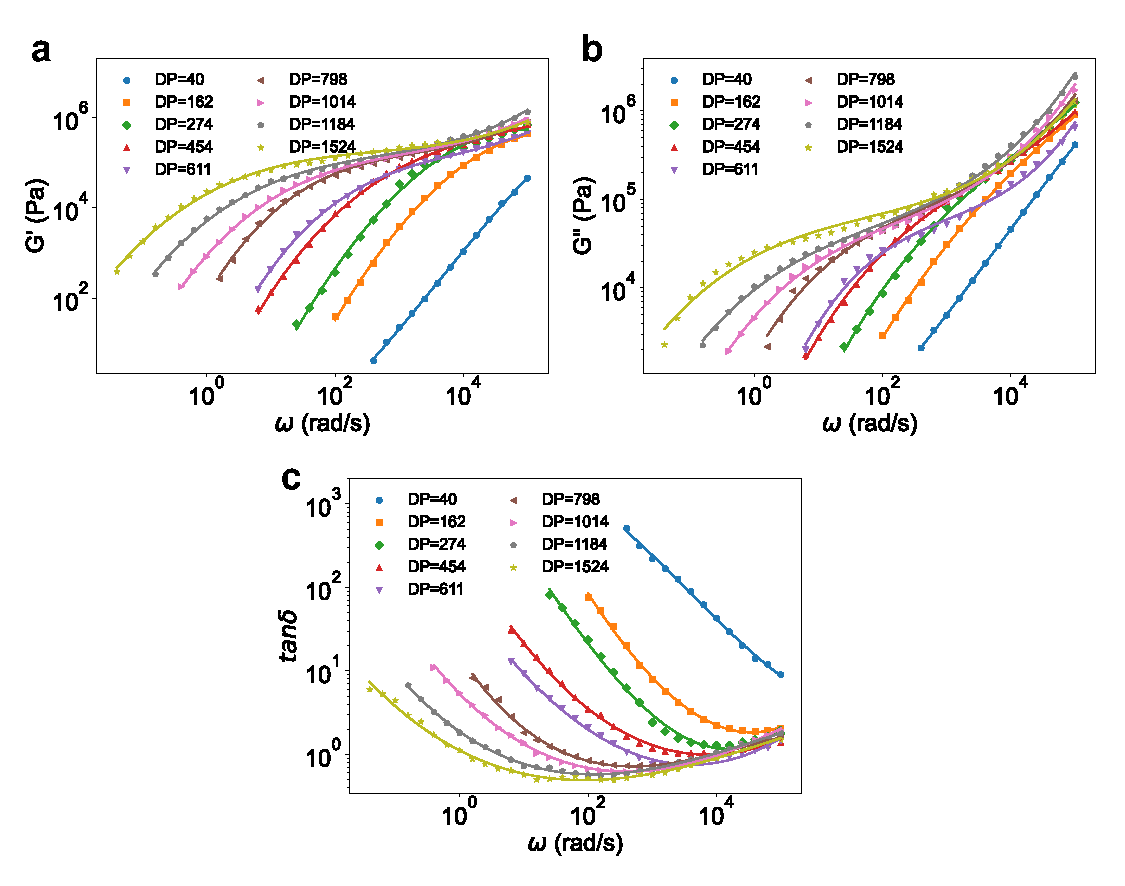
\includegraphics[width=0.8\textwidth]{Fig/pba-LF.pdf}
  \FigureBicaption{\label{pba-LF}不同PBA流体的频率-流变学性质参数数据低保真拟合结果:(a)不同DP值的PBA流体的频率-储存模量($\omega$-$\mathrm{G^{\prime}}$)数据拟合结果;(b)不同DP值的PBA流体的频率-损耗模量($\omega$-$\mathrm{G^{\prime\prime}}$)数据拟合结果;(c)不同DP值的PBA流体的频率-损耗角正切($\omega$-tan$\delta$)数据拟合结果}{Low-fidelity fitting results of frequency-rheological property parameter data of different PBA fluids: (a) Fitting results of frequency-storage modulus ($\omega$-$\mathrm{G^{\prime}}$) data of PBA fluids with different DP values; (b) Fitting results of frequency-loss modulus ($\omega$-$\mathrm{G^{\prime\prime}}$) data of PBA fluids with different DP values; (c) Fitting results of frequency-loss tangent ($\omega$-tan$\delta$) data of PBA fluids with different DP values}
\end{figure}
\begin{figure}[htbp]
  \centering
  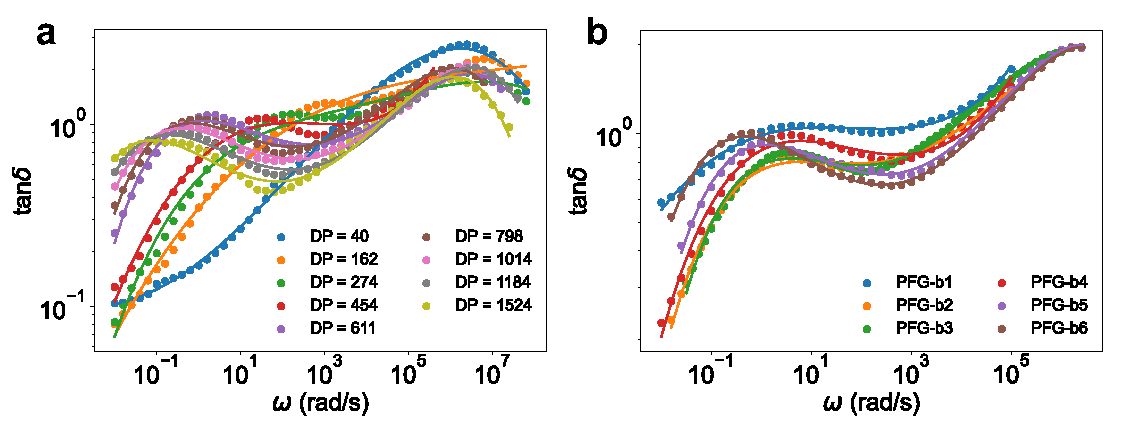
\includegraphics[width=0.8\textwidth]{Fig/pfgs-LF.pdf}
  \FigureBicaption{\label{pfgs-LF}不同PBA流体组合制备的PFGs的频率-流变学性质参数数据低保真拟合结果:(a)不同DP值的PBA流体制备的PFGs的频率-储存模量($\omega$-$\mathrm{G^{\prime}}$)数据拟合结果;(b)不同PBA流体组合制备的PFGs的频率-损耗模量($\omega$-$\mathrm{G^{\prime\prime}}$)数据拟合结果;(c)不同PBA流体组合制备的PFGs的频率-损耗角正切($\omega$-tan$\delta$)数据拟合结果}{Low-fidelity fitting results of frequency-rheological property parameter data of PFGs prepared by different PBA fluid combinations: (a) Fitting results of frequency-storage modulus ($\omega$-$\mathrm{G^{\prime}}$) data of PFGs prepared by PBA fluids with different DP values; (b) Fitting results of frequency-loss modulus ($\omega$-$\mathrm{G^{\prime\prime}}$) data of PFGs prepared by different PBA fluid combinations; (c) Fitting results of frequency-loss tangent ($\omega$-tan$\delta$) data of PFGs prepared by different PBA fluid combinations}
\end{figure}
本节采用Python的scipy.optimize库实现最小二乘法拟合,以公式\eqref{eq:doi-edwards-g1}和\eqref{eq:doi-edwards-g2}作为理论模型函数。首先对不同DP的PBA流体进行系统拟合,分析其频率-储存模量($\omega$-$\mathrm{G^{\prime}}$)、频率-损耗模量($\omega$-$\mathrm{G^{\prime\prime}}$)及频率-损耗角正切($\omega$-tan$\delta$)数据,拟合结果如图\ref{pba-LF}所示。从拟合曲线可观察到,模型对不同PBA流体的流变学特性表现出良好的拟合质量,曲线与实验数据点高度吻合。表\ref{LF-metrics-table}量化展示了低保真数据的回归拟合指标,其中$g_1$、$g_2$、$g_3$分别对应不同PBA流体的$\omega$-$\mathrm{G^{\prime}}$、$\omega$-$\mathrm{G^{\prime\prime}}$和$\omega$-tan$\delta$拟合结果。三组拟合的决定系数R$^2$均超过0.95,表明模型解释了数据变异性的95\%以上,拟合效果优异。
$g_1$组的MAPE为19.72\%,$g_2$组为15.89\%,$g_3$组为12.45\%,根据流变学数据分析的统计学标准,MAPE值小于20\%被认为处于可接受误差范围内,三组数据均满足此标准,适合用于后续深度学习模型的训练与验证。
\begin{table}
  \TableBicaption{\label{LF-metrics-table}低保真数据拟合回归指标表}{Regression Metrics of Low-Fidelity Data Fitting}  % 中英文标题
  \centering
  \small
  \begin{tabularx}{\textwidth}{>{\centering\arraybackslash}X >{\centering\arraybackslash}X >{\centering\arraybackslash}X >{\centering\arraybackslash}X} % 关键修改点
    \Xhline{1.5pt}
    实验分组  & R$^2$   & MAE       & MAPE(\%)                \tabularnewline
    \Xhline{0.5pt}  % 表头下方线
    $g_1$ & $0.977$ & $456.78$  & $19.72$ \tabularnewline
    $g_2$ & $0.982$ & $2456.23$ & $15.89 $ \tabularnewline
    $g_3$ & $0.964$ & $5.17$    & $12.45$ \tabularnewline
    $g_4$ & $0.985$ & $0.25$    & $19.91$\tabularnewline
    $g_5$ & $0.962$ & $0.11$    & $9.89$\tabularnewline
    \Xhline{1.5pt}
  \end{tabularx}
\end{table}

随后,针对PBA流体注入制备的PFGs体系进行拟合分析。图\ref{pfgs-LF}(a)呈现了不同DP值PBA注入制备的PFGs数据的拟合曲线,模型捕捉到了材料在频率域内的流变响应特征,拟合曲线与实验数据点表现出高度一致性。该拟合对应的定量评估指标见表\ref{LF-metrics-table}中的$g_4$项,R$^2$值达0.985,MAPE值为19.91\%,处于可接受的误差范围内,证实了模型对单组分PBA注入PFGs流变行为的有效描述能力。

图\ref{pfgs-LF}(b)展示了多分子量PBA组合注入制备的PFGs数据拟合结果,其中b1-b6代表不同的PBA流体组合配方,详细组合参数见表\ref{pba-com-groups}。拟合曲线显示模型成功捕捉了多组分体系中的复杂流变学行为,定量评估指标如表\ref{LF-metrics-table}中$g_5$项所示,R$^2$值为0.962,MAPE值仅为9.89\%,误差显著低于单组分体系,表明理论模型对多组分PFGs体系具有更高的预测精度,为后续深入研究多组分体系的流变学特性奠定了坚实基础。


% 单PBA流体本构建模
\subsection{单PBA流体本构建模}
本节首先对不同分子量的单PBA流体进行深度学习本构建模,分别预测$\mathrm{G^{\prime}}$、$\mathrm{G^{\prime\prime}}$和tan$\delta$。图\ref{pba-g1}展示了$\mathrm{G^{\prime}}$的预测结果,其中图\ref{pba-g1}(a)为真实值-预测值对比曲线。从图中可观察到,PINN模型的预测曲线相较于DNN模型更贴近真实数据点,表现出更优的拟合效果。图\ref{pba-g1}(b)的残差分析显示,PINN预测值的残差分布更为集中于零值附近,且极值范围明显小于DNN模型。这些观察结果定性表明PINN在该任务上具有更强的泛化预测能力。
\begin{figure}[htbp]
  \centering
  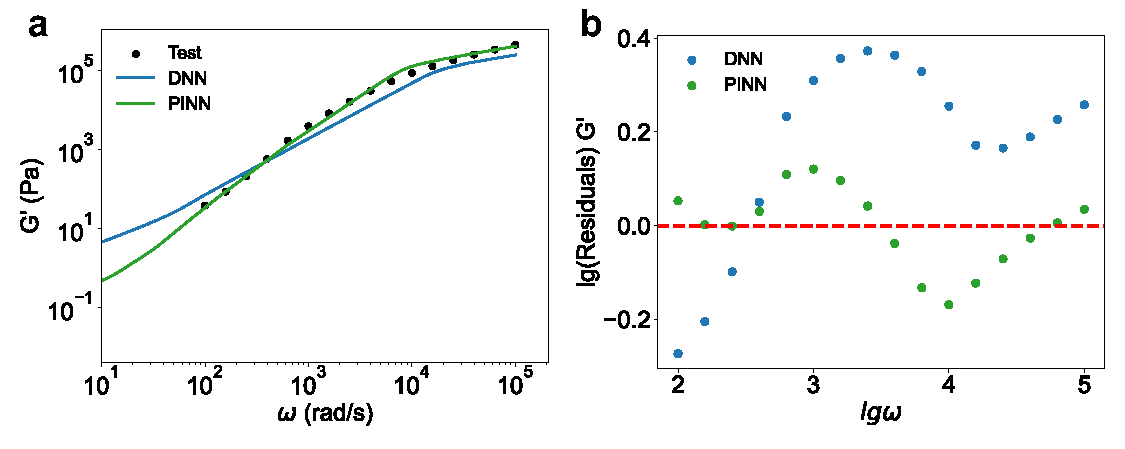
\includegraphics[width=0.8\textwidth]{Fig/pba-g1.pdf}
  \FigureBicaption{\label{pba-g1}不同分子量PBA流体的$\mathrm{G^{\prime}}$预测结果对比(PINN vs. DNN):(a)真实值-预测值对比曲线;(b)残差分布图}{Comparative prediction results of $\mathrm{G^{\prime}}$ for PBA fluids with different molecular weights (PINN vs. DNN): (a) True-predicted value comparison curves; (b) Residual distribution plot}
\end{figure}

图\ref{pba-g2}呈现了$\mathrm{G^{\prime\prime}}$的预测结果,图\ref{pba-g2}(a)为真实值-预测值对比曲线。分析表明,PINN模型的预测值序列与真实值分布趋势呈现高度一致性,而DNN模型在低频率区域存在明显的系统性高估现象。残差分布图(图\ref{pba-g2}(b))进一步证实,PINN模型的残差绝对值显著低于DNN模型,且分布更为集中于零值附近。这些证据共同表明PINN模型在$\mathrm{G^{\prime\prime}}$预测任务上具有更优的泛化性能。
\begin{figure}[htbp]
  \centering
  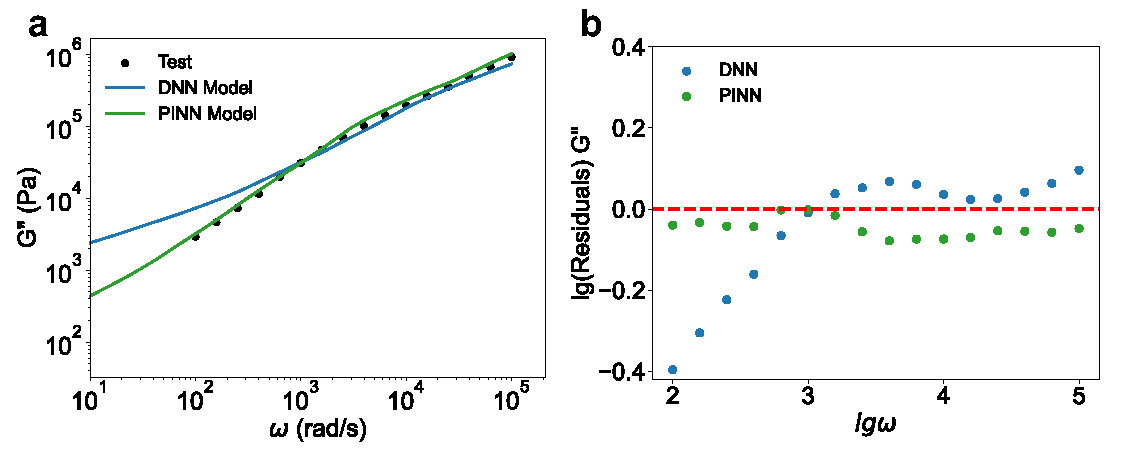
\includegraphics[width=0.8\textwidth]{Fig/pba-g2.pdf}
  \FigureBicaption{\label{pba-g2}不同分子量PBA流体的$\mathrm{G^{\prime\prime}}$预测结果对比(PINN vs. DNN):(a)真实值-预测值对比曲线;(b)残差分布图}{Comparative prediction results of $\mathrm{G^{\prime\prime}}$ for PBA fluids with different molecular weights (PINN vs. DNN): (a) True-predicted value comparison curves; (b) Residual distribution plot}
\end{figure}
\begin{figure}[htbp]
  \centering
  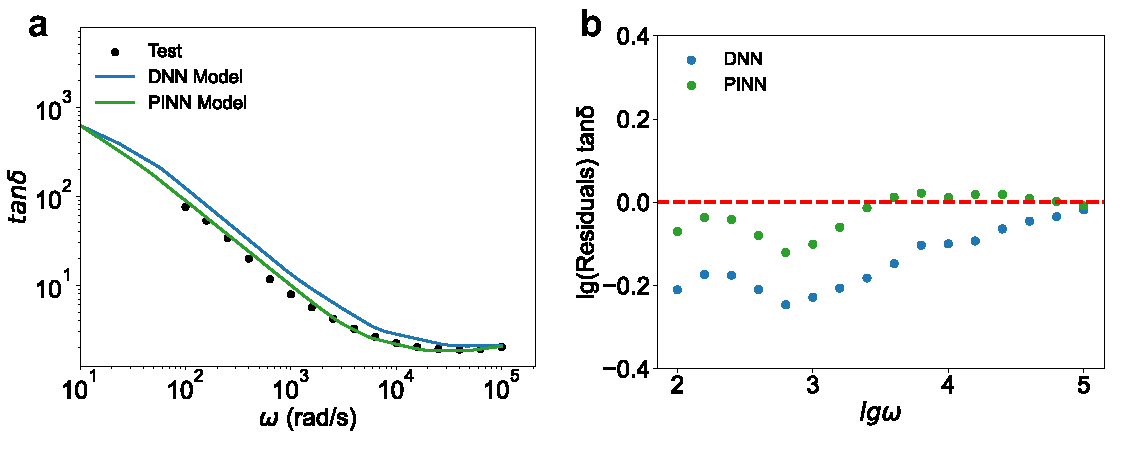
\includegraphics[width=0.8\textwidth]{Fig/pba-lossf.pdf}
  \FigureBicaption{\label{pba-lossf}不同分子量PBA流体的tan$\delta$预测结果对比(PINN vs. DNN):(a)真实值-预测值对比曲线;(b)残差分布图}{Comparative prediction results of tan$\delta$ for PBA fluids with different molecular weights (PINN vs. DNN): (a) True-predicted value comparison curves; (b) Residual distribution plot}
\end{figure}
\begin{figure}[htbp]
  \centering
  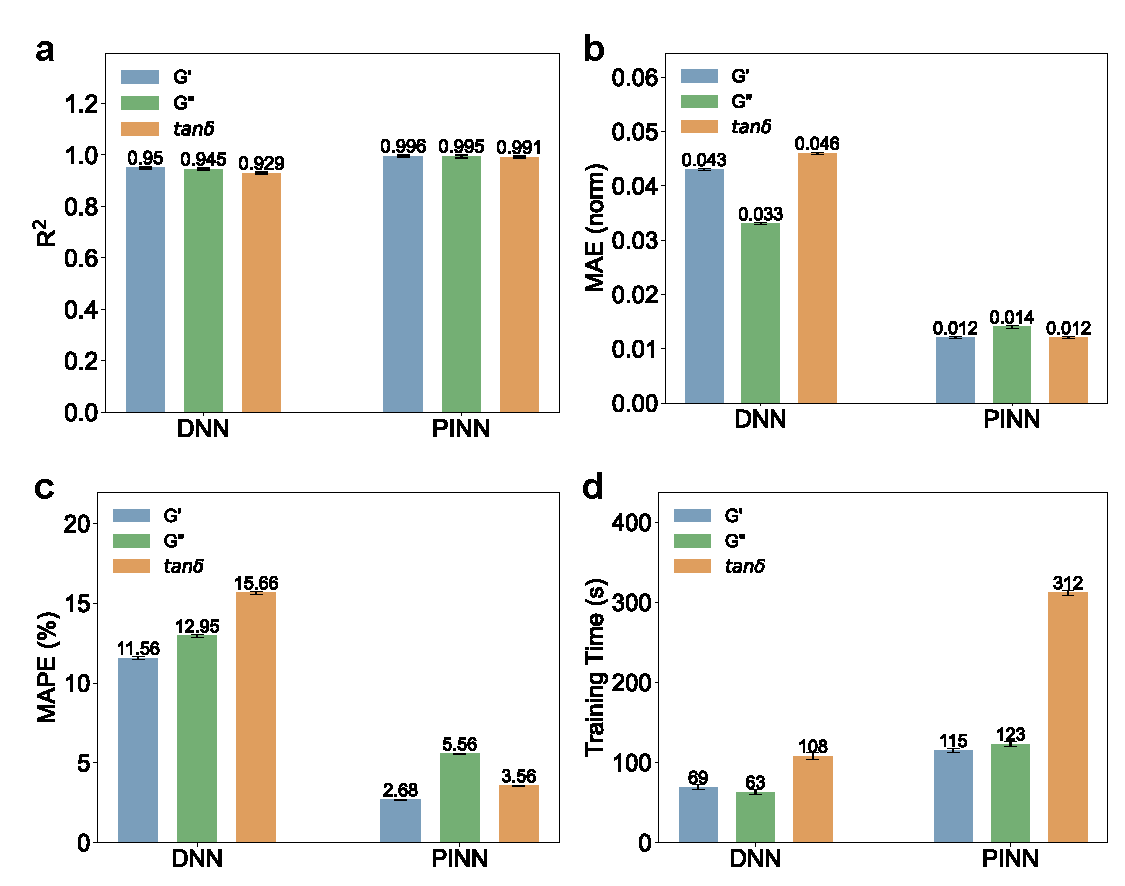
\includegraphics[width=0.8\textwidth]{Fig/pba-metrics.pdf}
  \FigureBicaption{\label{pba-metrics}不同分子量PBA流体模型性能指标对比(PINN vs. DNN):(a)决定系数R$^2$;(b)平均绝对误差MAE;(c)平均绝对百分比误差MAPE;(d)训练时间}{Performance metrics comparison for PBA fluids modeling (PINN vs. DNN): (a) Coefficient of determination R$^2$; (b) Mean absolute error MAE; (c) Mean absolute percentage error MAPE; (d) Training time}
\end{figure}
图\ref{pba-lossf}展示了tan$\delta$的预测结果,图\ref{pba-lossf}(a)为真实值-预测值对比曲线。观察发现,PINN模型的预测轨迹与实验数据点吻合度高,展现出优异的轨迹跟踪特性。残差分布图(图\ref{pba-lossf}(b))显示,尽管两种模型的预测残差均呈现负偏差为主的分布特征,但PINN模型的残差绝对值和极值均显著小于DNN模型,表明其预测精度更高。

为定量评估PBA流体模量数据的建模效果,本节计算了测试集上的R$^2$、MAE、MAPE及训练时间。图\ref{pba-metrics}展示了两种模型在三项预测任务上的性能指标对比。结果表明,PINN模型在$\mathrm{G^{\prime}}$、$\mathrm{G^{\prime\prime}}$和tan$\delta$三个任务上的R$^2$值均略高于DNN模型,表明其对数据变异性的解释能力更强。在误差指标方面,PINN模型的MAE值在所有任务中均显著低于DNN模型,而MAPE值均控制在10\%以下,处于高精度预测范围。相比之下,DNN模型的MAPE值均超过10\%,预测精度较低。然而,PINN模型的训练时间约为DNN模型的$2\sim3$倍,这是由于物理约束引入的额外计算复杂度所致。

这些结果证实,PINN通过将物理守恒方程嵌入为正则化约束,有效抑制了纯数据驱动模型易发生的过拟合现象。残差分布的紧致性和对称性改善进一步验证了物理先验知识对模型泛化能力的显著提升。综合可视化分析与统计指标可知,在本研究涉及的偏微分方程反演任务中,PINN框架通过融合物理机理与数据特征的双重驱动机制,实现了比传统数据驱动范式更优的泛化预测性能。
% PBA嵌入PFGs
\subsection{单组分PBA注入的PFGs本构建模}
本节对第二类数据,即单一分子量PBA注入制备的PFGs进行深度学习本构建模,探究在不同分子量PBA注入的PFGs上,PINN模型与DNN模型的性能对比。图\ref{pfgs-single}为两种算法模型对这类数据的预测性能对比。图\ref{pfgs-single}(a)为真实值-预测值曲线,这里对比的是tan$\delta$的预测结果。从图中可以看出,PINN模型的预测曲线与真实值曲线更为贴近,拟合效果更佳。图\ref{pfgs-single}(b)为残差图,PINN模型的残差绝对值显著低于DNN模型的残差绝对值,PINN的残差更为邻近0刻度线。综上所述,可以定性认为在此项任务中,PINN模型的泛化预测效果更佳。
\begin{figure}[htbp]
  \centering
  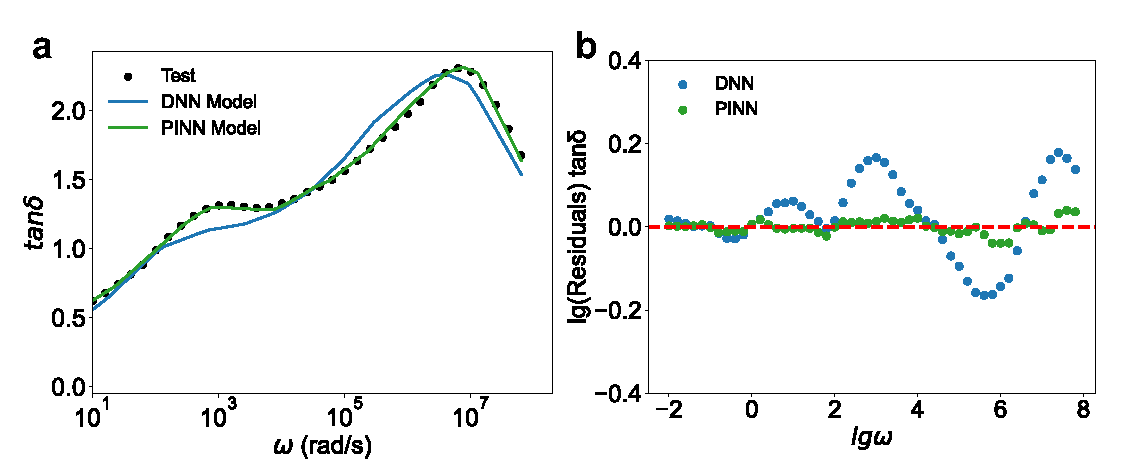
\includegraphics[width=0.8\textwidth]{Fig/pfgs-single.pdf}
  \FigureBicaption{\label{pfgs-single}单分子量PBA注入的PFGs数据PINN和DNN建模的tan$\delta$预测结果:(a)PINN和DNN在测试集上的预测值与真实值对比曲线;(b)PINN和DNN在测试集上的预测值残差图}{Prediction results of tan$\delta$ of PFGs prepared by single molecular weight PBA injection using PINN and DNN modeling: (a) Comparison curves of predicted vs. true values for PINN and DNN on test set; (b) Residual plots of predicted values for PINN and DNN on test set}
\end{figure}
为了进一步定量分析单组分PBA注入的PFGs数据的PINN建模效果,本节计算测试集的R$^2$、MAE、MAPE、Training Time。图\ref{pfgs-single-metrics}为两个模型tan$\delta$预测的指标对比图。从图中可以看出,PINN模型在该任务上的R$^2$略低于DNN模型。在MAE指标上,PINN为0.012,DNN为0.071,PINN的MAE值相比DNN降低了83.38\%。MAPE指标方面,PINN为0.03\%,DNN为8.59\%,相差近3个数量级别。这里PINN模型的R$^2$值意外地低可能是因为PINN引入的物理约束可能降低了模型对训练数据的过拟合程度,但模型的泛化能力和实际预测精度(MAPE)更好这些结果表明,PINN模型在预测单组分PBA注入的PFGs流变性能时具有更高的准确性和稳定性。然而,与前文类似,PINN模型的训练时间显著长于DNN模型,大约是后者的5倍,这是由于物理约束的引入增加了计算复杂度。
\begin{figure}[htbp]
  \centering
  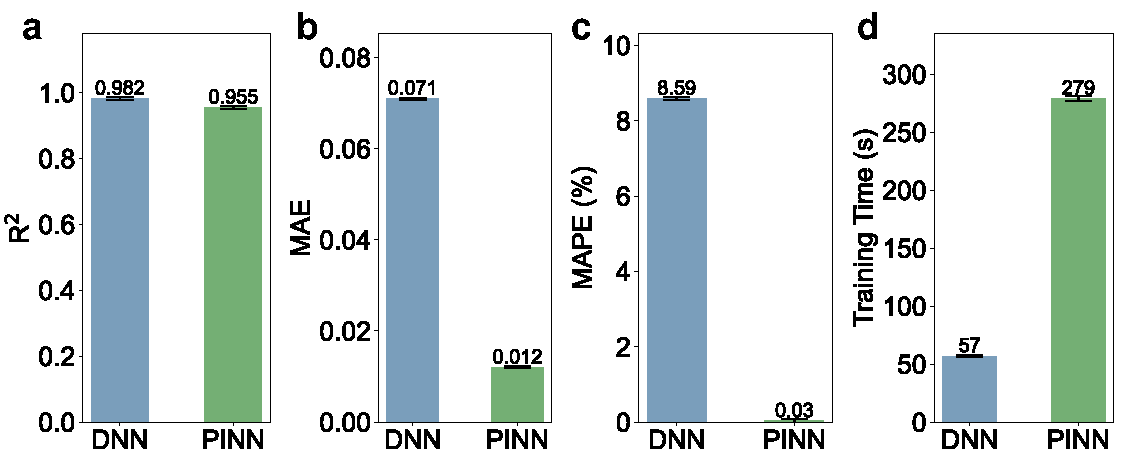
\includegraphics[width=0.8\textwidth]{Fig/pfgs-single-metrics.pdf}
  \FigureBicaption{\label{pfgs-single-metrics}单分子量PBA注入的PFGs数据PINN和DNN建模的tan$\delta$预测指标对比图:(a)R$^2$值;(b)MAE值;(c)MAPE值;(d)训练时间}{Comparison of R$^2$, MAE, MAPE, and Training Time metrics of PINN and DNN for tan$\delta$ prediction of PFGs prepared by single molecular weight PBA injection: (a) R$^2$ value; (b) MAE value; (c) MAPE value; (d) Training Time}
\end{figure}
综上所述,PINN模型在单组分PBA注入的PFGs数据的建模预测中展现出显著优势。从定性分析角度来看,PINN模型生成的预测曲线与实验数据点更为贴合,残差分布更加集中且接近零值。从定量分析的角度来看,尽管PINN的R²指标略低于DNN模型,但在MAE和MAPE这两个更能反映实际预测精度的指标上,PINN模型都取得了显著优势。特别是在MAPE指标上,PINN与DNN指标差近3个数量级。这表明PINN通过引入物理约束,有效抑制了过拟合现象,提高了模型的泛化能力和预测准确性。然而需要注意的是,由于引入物理约束增加了计算复杂度,PINN模型的训练时间约为DNN模型的5倍,这是可以预见的成本增加。

\subsection{多组分PBA注入的PFGs本构建模}
上一节研究了单组分PBA注入的PFGs数据建模,验证了PINN模型在处理简单制备参数特征(单一分子量)时,通过引入物理约束能够有效提升模型的泛化能力。本节将进一步探讨PINN模型在多组分PBA注入的PFGs数据上的表现,研究其在处理复杂制备参数特征(多分子量组合)时的泛化性能,以期为实际应用提供更具参考价值的理论基础。
\begin{figure}[htbp]
  \centering
  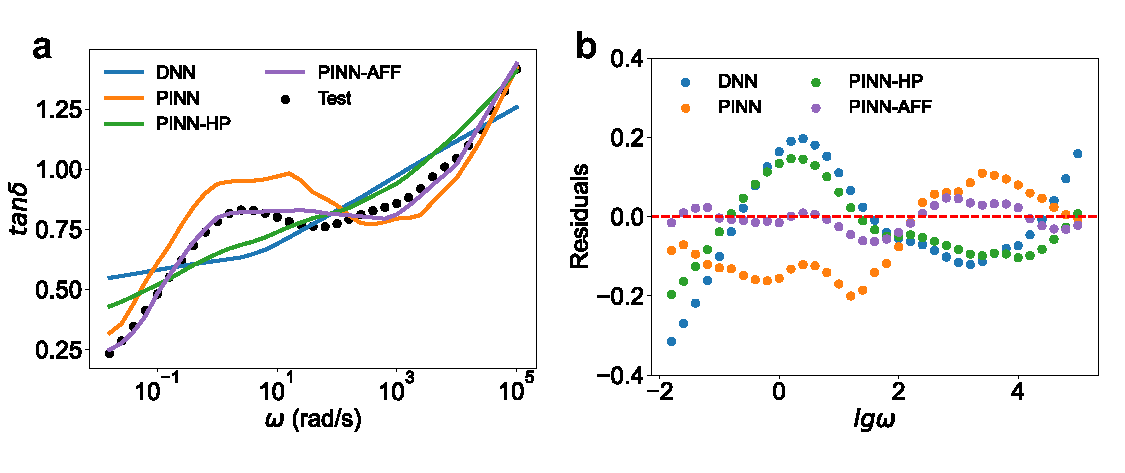
\includegraphics[width=0.8\textwidth]{Fig/pfgs-com.pdf}
  \FigureBicaption{\label{pfgs-com}多组分PBA注入制备的PFGs数据不同算法建模的tan$\delta$预测结果:(a)不同算法在测试集上的预测值与真实值对比曲线;(b)不同算法在测试集上的预测值残差图}{Prediction results of tan$\delta$ of PFGs prepared by multiple molecular weight PBA injection using different algorithms: (a) Comparison curves of predicted vs. true values on test set; (b) Residual plots of predicted values on test set}
\end{figure}
图\ref{pfgs-com}呈现了多组分PBA注入的PFGs数据建模结果,其中图\ref{pfgs-com}(a)为真实值-预测值对比曲线,图\ref{pfgs-com}(b)展示残差分布。本研究采用四种不同算法进行建模对比:DNN、PINN、基于哈达玛积特征融合的物理信息神经网络(Physics-informed Neural Network with Hadamard Product, PINN-HP)以及基于注意力机制特征融合的物理信息神经网络(Physics-informed Neural Network with Attention Feature Fusion, PINN-AFF)。从图\ref{pfgs-com}可明显观察到PINN-AFF模型表现最为优异,其预测曲线与实验数据曲线高度吻合,残差分布极为集中且紧密围绕零值轴线。相比之下,其他算法模型的预测结果均呈现不同程度的系统性偏差。

\begin{figure}[htbp]
  \centering
  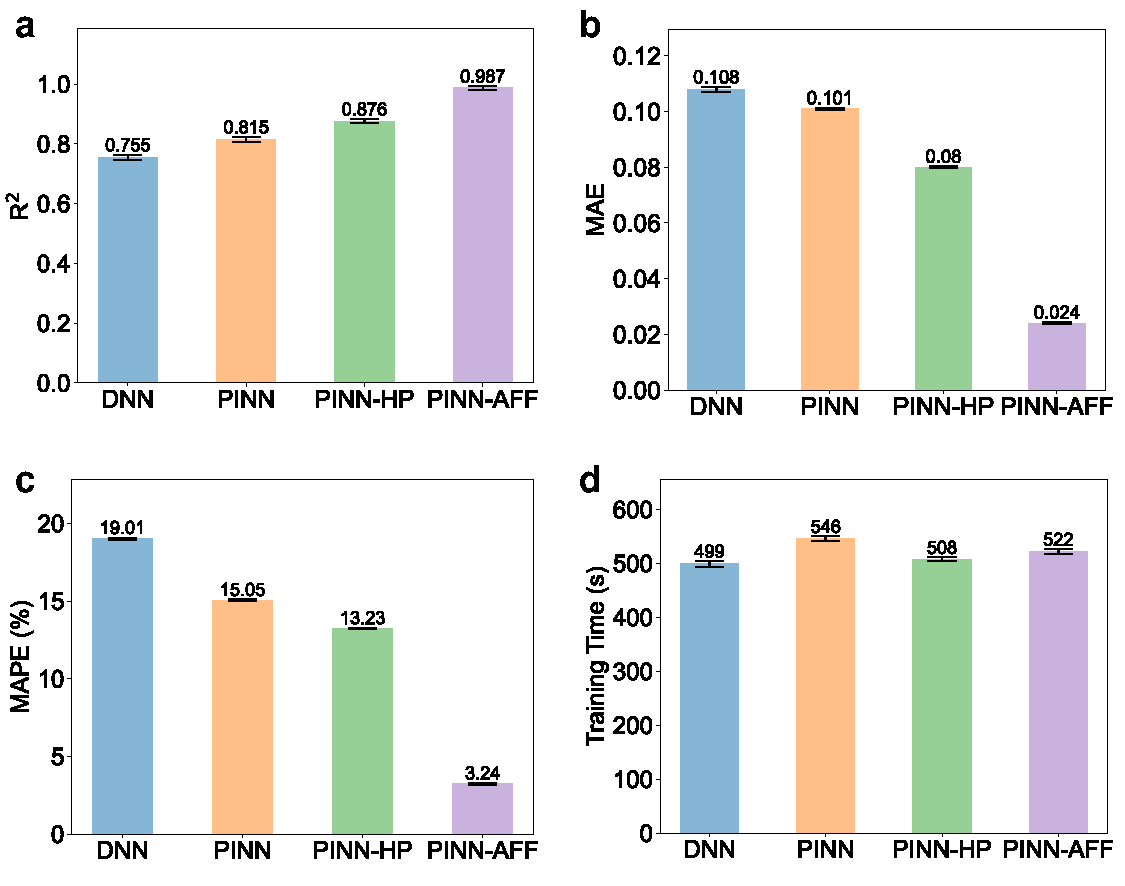
\includegraphics[width=0.8\textwidth]{Fig/pfgs-com-metrics.pdf}
  \FigureBicaption{\label{pfgs-com-metrics}多组分PBA注入制备的PFGs数据不同算法建模的tan$\delta$预测指标对比图:(a)R$^2$ 值;(b)MAE 值;(c)MAPE 值;(d)训练时间}{Comparison of R$^2$, MAE, MAPE, and Training Time metrics of PINN and DNN for tan$\delta$ prediction of PFGs prepared by multiple molecular weight PBA injection: (a) R$^2$ value; (b) MAE value; (c) MAPE value; (d) Training Time}
\end{figure}
为进一步量化多组分PBA注入的PFGs数据的PINN建模效能,本节计算了测试集上的R$^2$、MAE、MAPE及训练时间评价指标。图\ref{pfgs-com-metrics}展示了四种算法模型在tan$\delta$预测任务上的性能对比。从定量指标分析可见,PINN-AFF模型在所有评价维度上均表现最佳,PINN-HP模型次之,标准PINN模型再次,而传统DNN模型表现最为欠佳。这一结果证实,引入特征融合机制能够显著增强PINN模型的预测性能,尤其是基于注意力机制的特征融合策略效果最为显著。从计算效率角度分析,PINN系列模型的训练时间普遍长于DNN模型,这与物理约束引入带来的额外计算负荷相关。值得注意的是,PINN-HP模型的训练时间略低于标准PINN,这归因于哈达玛积特征融合降低了特征维度,从而减少了模型参数量;而PINN-AFF的训练时间略高于PINN-HP,这是由于注意力机制引入的计算复杂度增加所致。


综合图\ref{pfgs-com}和图\ref{pfgs-com-metrics}的分析结果可知,在处理高维特征空间且特征间存在复杂物理耦合关系的场景下,标准PINN模型的学习泛化能力面临一定局限。针对这一挑战,本研究提出了两种改进方案:首先,PINN-HP模型通过哈达玛积运算实现分子量与组分含量特征的乘性融合,这种方式相当于为模型预设了特征间的物理相互作用形式,从而提升了模型对复杂流变学行为的表征能力。在此基础上,PINN-AFF模型进一步引入注意力机制,对不同分子量与组分含量的联合特征实施自适应加权。这种机制能够精确学习不同高分子链段间的相互作用模式,通过注意力分数定量表征组分间流变学相互作用强度,并能自动识别主导组分的影响程度,例如能够有效捕捉高分子量组分对整体流变学特性的决定性贡献。实验结果表明,这两种改进方案均显著提升了模型性能,其中PINN-AFF模型在多组分PFGs流变学预测任务中取得了最优效果。

% CVAE组分预测
\subsection{CVAE组分预测的多模态解分析}

本节探索了使用CVAE模型从材料的流变学性质反向预测其组分配比的可行性。基于训练完成的生成模型,我们输入目标流变学参数[$\omega$,$\mathrm{G^{\prime}}$,$\mathrm{G^{\prime\prime}}$,tan$\delta$],生成100组多模态解,并对生成结果进行系统的残差分析。
\begin{figure}[htbp]
  \centering
  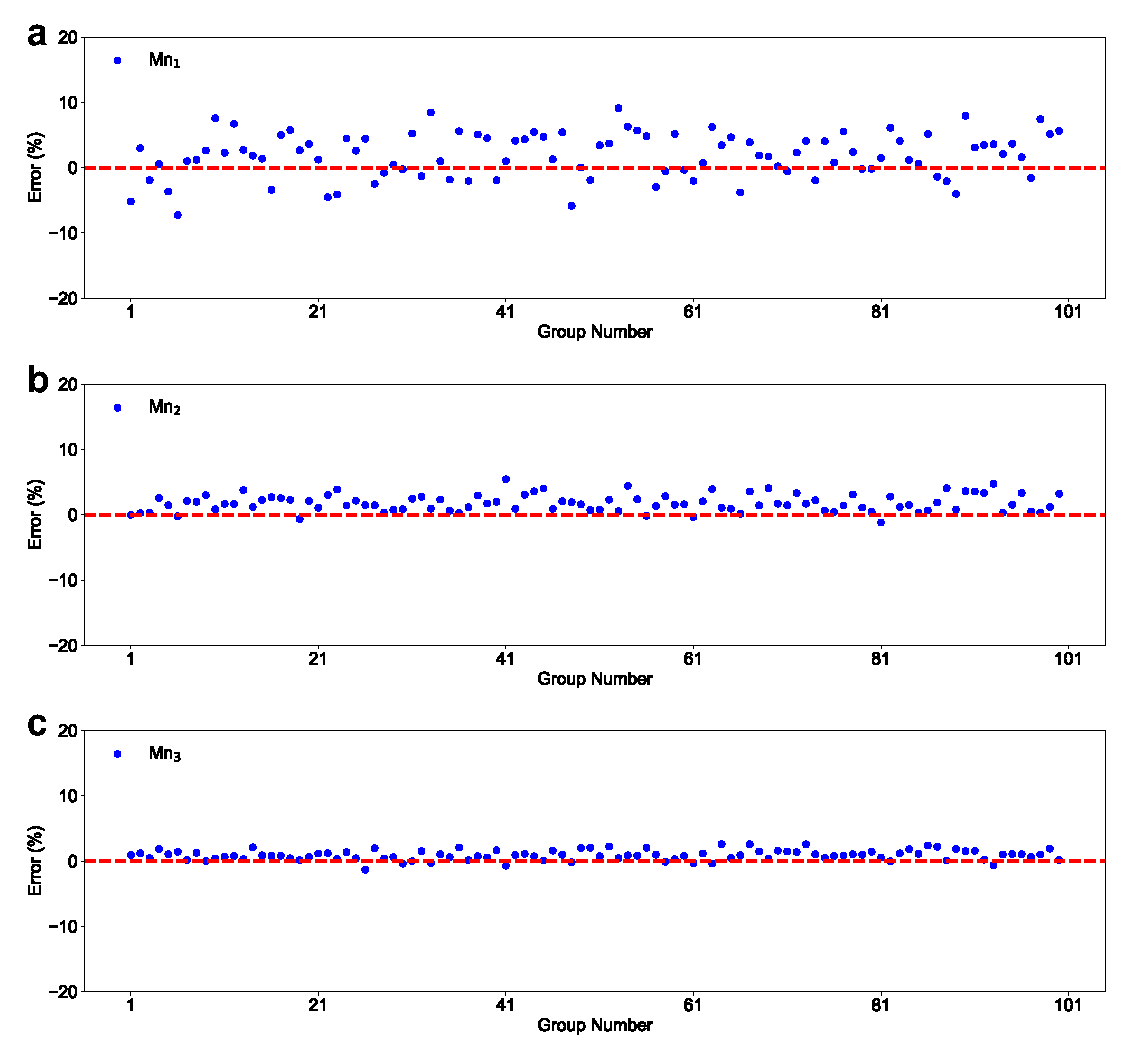
\includegraphics[width=0.8\textwidth]{Fig/reverse-redisual-Mn.pdf}
  \FigureBicaption{\label{reverse-redisual-Mn}CVAE生成的100组多模态解中不同分子量组分Mn$_1$、Mn$_2$、Mn$_3$的残差分布:(a)Mn$_1$残差分布;(b)Mn$_2$残差分布;(c)Mn$_3$残差分布}{Residual distributions of 100 multimodal solutions generated by CVAE for different molecular weight components Mn$_1$, Mn$_2$, Mn$_3$: (a) Residual distribution of Mn$_1$; (b) Residual distribution of Mn$_2$; (c) Residual distribution of Mn$_3$}
\end{figure}

\begin{figure}[htbp]
  \centering
  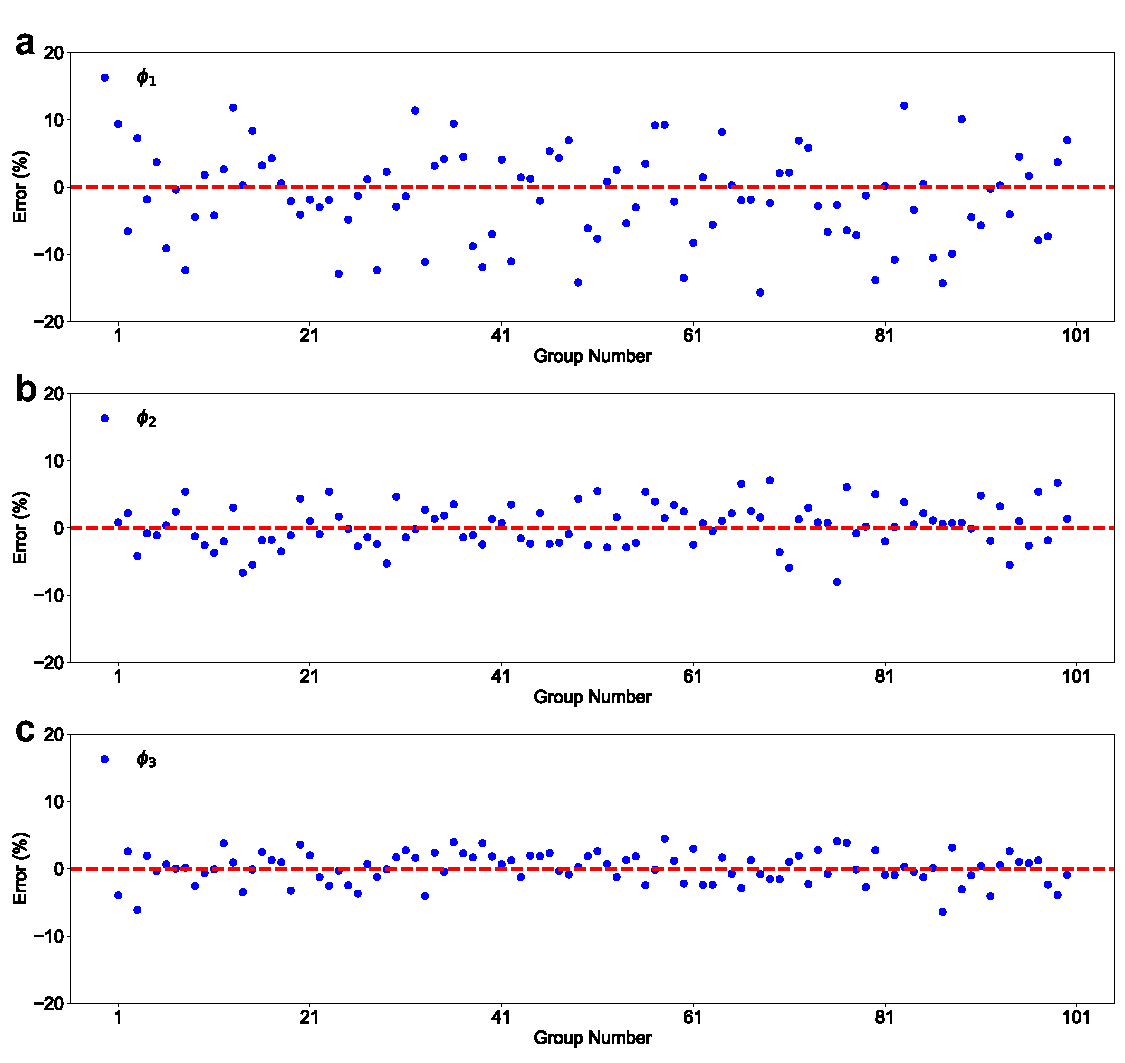
\includegraphics[width=0.8\textwidth]{Fig/reverse-redisual-phi.pdf}
  \FigureBicaption{\label{reverse-redisual-phi}CVAE生成的100组多模态解中不同组分含量$\phi_1$、$\phi_2$、$\phi_3$的残差分布:(a)$\phi_1$残差分布;(b)$\phi_2$残差分布;(c)$\phi_3$残差分布}{Residual distributions of 100 multimodal solutions generated by CVAE for different component contents $\phi_1$, $\phi_2$, $\phi_3$: (a) Residual distribution of $\phi_1$; (b) Residual distribution of $\phi_2$; (c) Residual distribution of $\phi_3$}
\end{figure}
图\ref{reverse-redisual-Mn}展示了分子量参数Mn的残差分布。结果表明,三种分子量组分Mn$_1$、Mn$_2$、Mn$_3$的残差均呈现正态分布特征,最大偏差约为10\%,处于可接受范围内。残差大小依次为Mn$_1$>Mn$_2$>Mn$_3$。图\ref{reverse-redisual-phi}则显示了组分含量参数$\phi$的残差分布。$\phi_1$、$\phi_2$、$\phi_3$同样呈现正态分布特征,最大偏差约为20\%,残差大小顺序为$\phi_1$>$\phi_2$>$\phi_3$。

值得注意的是,在测试集中Mn$_1$<Mn$_2$<Mn$_3$,$\phi_1$<$\phi_2$<$\phi_3$,由此观察到残差大小与参数实际值呈现负相关关系 - 即参数绝对值越小,其预测误差反而越大。这一现象揭示了模型在预测较小数值参数时的精度局限性,实际应用时,可以通过调整量纲一定程度缓解这一问题。
\begin{figure}[htbp]
  \centering
  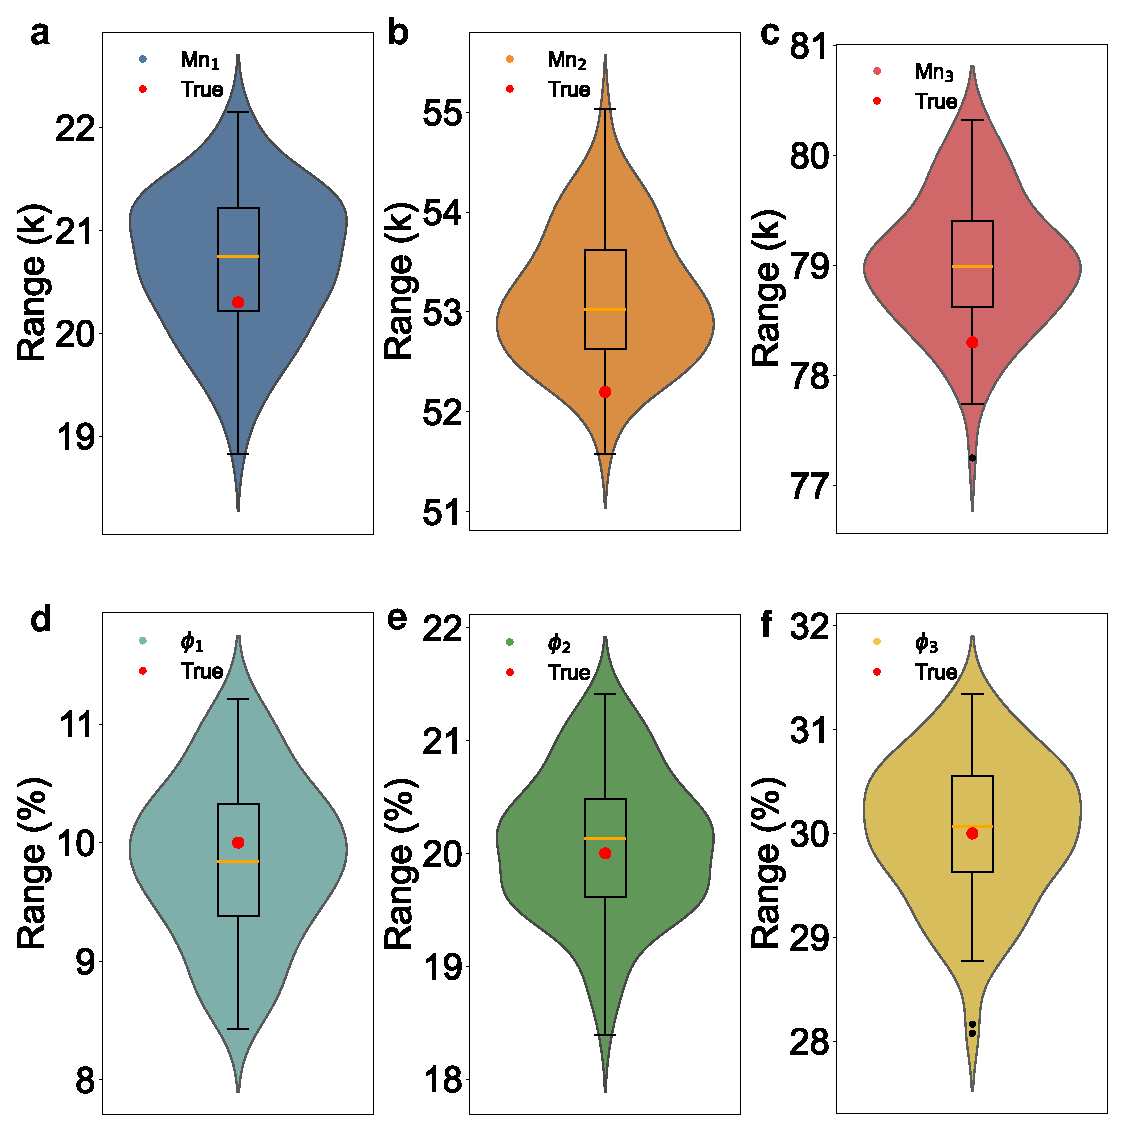
\includegraphics[width=0.8\textwidth]{Fig/reverse-violin.pdf}
  \FigureBicaption{\label{reverse-violin}CVAE生成的100组多模态解的violin图:(a)分子量参数Mn$_1$的多模态解分布;(b)分子量参数Mn$_2$的多模态解分布;(c)分子量参数Mn$_3$的多模态解分布;(d)组分含量参数$\phi_1$的多模态解分布;(e)组分含量参数$\phi_2$的多模态解分布;(f)组分含量参数$\phi_3$的多模态解分布}{Violin plots of 100 multimodal solutions generated by CVAE: (a) Distribution of multimodal solutions for molecular weight parameter Mn$_1$; (b) Distribution of multimodal solutions for molecular weight parameter Mn$_2$; (c) Distribution of multimodal solutions for molecular weight parameter Mn$_3$; (d) Distribution of multimodal solutions for component content parameter $\phi_1$; (e) Distribution of multimodal solutions for component content parameter $\phi_2$; (f) Distribution of multimodal solutions for component content parameter $\phi_3$}
\end{figure}

图\ref{reverse-violin}为生成数据的violin图。(a-f)分别展示了分子量参数Mn$_1$、Mn$_2$、Mn$_3$和组分含量参数$\phi_1$、$\phi_2$、$\phi_3$的多模态解分布情况。由图可见,真实分子量数据(Mn)位于生成分子量数据的下四分位数附近,整体上生成值偏大,但大部分数据分布在中位数附近;而真实组分含量数据($\phi$)则位于生成组分含量数据中位数附近,总体生成效果良好。从核密度曲线形态来看,所有参数分布均呈现出中间宽、两端窄的典型小提琴形状,表明数据分布集中且符合正态分布特征,无明显多峰值现象。

通过分析各参数核密度曲线最宽处与中位数线的相对位置发现:Mn$_1$的核密度曲线最宽处位于中位数线上方,表明生成数据相对真实值略有高估;Mn$_2$的核密度曲线最宽处位于中位数线下方,显示生成数据略低于中位数水平;而其余各参数(Mn$_3$、$\phi_1$、$\phi_2$、$\phi_3$)的核密度曲线最宽处与中位数线基本重合,说明这些参数的生成分布更为准确。异常点分析结果显示,所有参数的异常点数量均较少,进一步证实了生成数据的整体质量较高。
\begin{figure}[htbp]
  \centering
  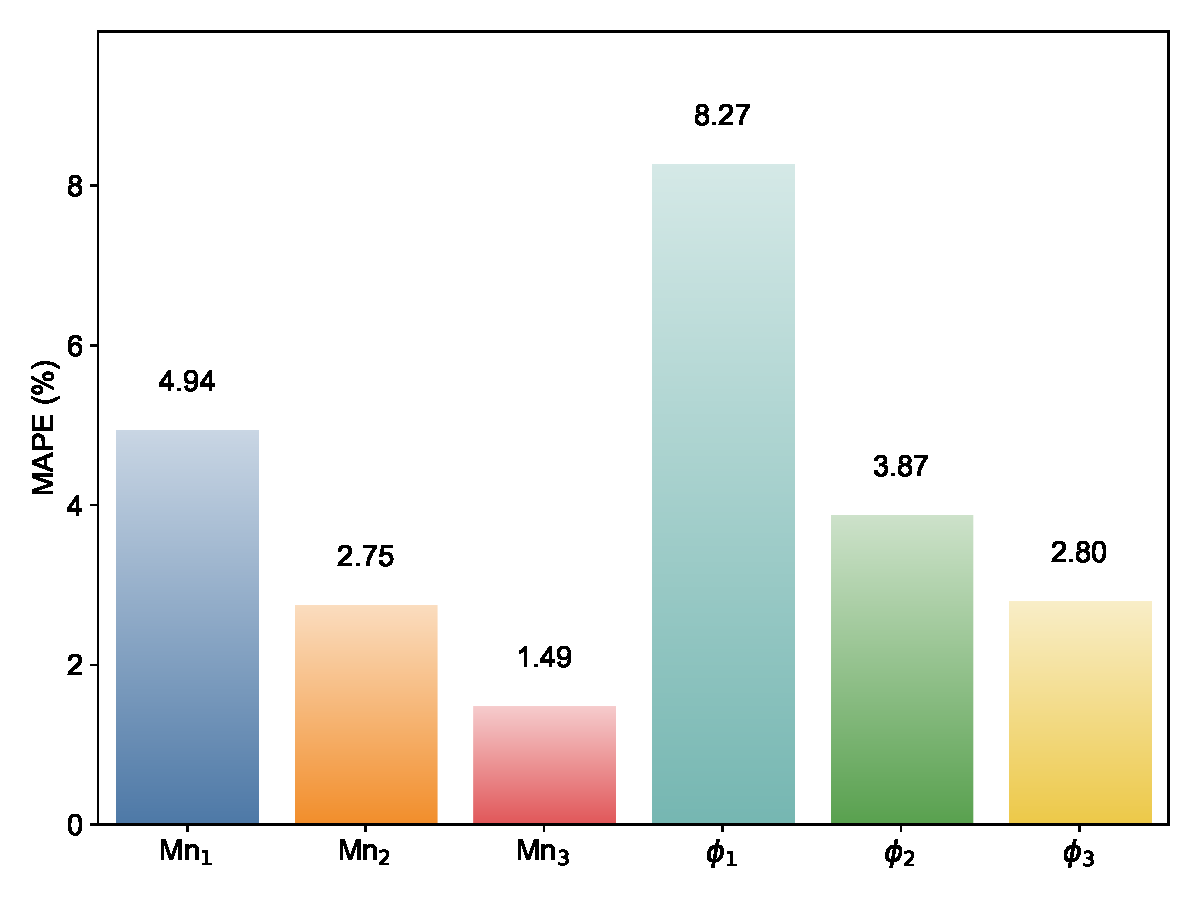
\includegraphics[width=0.8\textwidth]{Fig/MAPE_bar_chart.pdf}
  \FigureBicaption{\label{reverse-mape}CVAE生成的100组多模态解中分子量参数Mn$_1$、Mn$_2$、Mn$_3$和组分含量参数$\phi_1$、$\phi_2$、$\phi_3$的MAPE图}{MAPE chart of molecular weight parameters Mn$_1$, Mn$_2$, Mn$_3$ and component content parameters $\phi_1$, $\phi_2$, $\phi_3$ of 100 multimodal solutions generated by CVAE}
\end{figure}

图\ref{reverse-mape}展示了各参数的MAPE值。分子量参数Mn$_1$、Mn$_2$、Mn$_3$的MAPE值分别为4.94\%、2.75\%、1.49\%,组分含量参数$\phi_1$、$\phi_2$、$\phi_3$的MAPE值分别为8.27\%、3.87\%、2.80\%。这些数据揭示了几个重要趋势:首先,分子量参数的预测精度总体优于组分含量参数,表明模型在预测分子量特征时具有更好的准确性;其次,无论是分子量还是组分含量参数,都呈现出随着数值增大(即Mn$_1$ < Mn$_2$ < Mn$_3$和$\phi_1$ < $\phi_2$ < $\phi_3$)预测误差逐渐减小的规律,这与前述残差分析结果一致。值得注意的是,即使是预测误差最大的$\phi_1$,其MAPE值也仅为8.27\%,而其他参数的MAPE值均控制在5\%以内,说明模型整体预测精度达到了较高水平,具有良好的实用价值。

综合以上分析,CVAE模型在从流变学性质反向预测组分配比的任务中展现出了良好性能。通过多维度评估可得出以下结论:首先,模型生成的组分配比数据整体呈现正态分布特征,预测结果分布集中且稳定,异常值少;其次,预测误差随参数数值增大而减小,这一特征在分子量和组分含量两类参数中均有体现,可能源于数据标准化过程中较小数值参数更易受到舍入和归一化误差影响;第三,从MAPE指标来看,分子量参数的预测精度普遍优于组分含量参数,但两类参数的预测误差均控制在可接受范围内(最大MAPE为8.27\%)。这些结果表明,CVAE模型能够有效实现从材料性质到材料制备参数的反向设计,为高分子材料配方开发提供了一种可靠的数据驱动方法。

\subsection{正逆向联合建模分析}

上一节通过分析CVAE生成的100组组分数据与真实组分数据的误差来评估CVAE模型的生成效果,但这种分析方法存在明显的局限性。首先,组分数据与频率-损耗角正切曲线之间存在多对一的映射关系,即理论上可能存在多种不同的组分配比,所制备的材料却具有相同或近似的频率-损耗角正切曲线。这种多解性是高分子材料设计中的普遍现象,源于不同分子量组分之间复杂的相互作用机制。其次,组分配比的微小变化可能导致材料性能的显著差异,这种非线性关系使得仅通过比较组分数据误差来评估模型效果是不够全面和准确的。
\begin{figure}[htbp]
  \centering
  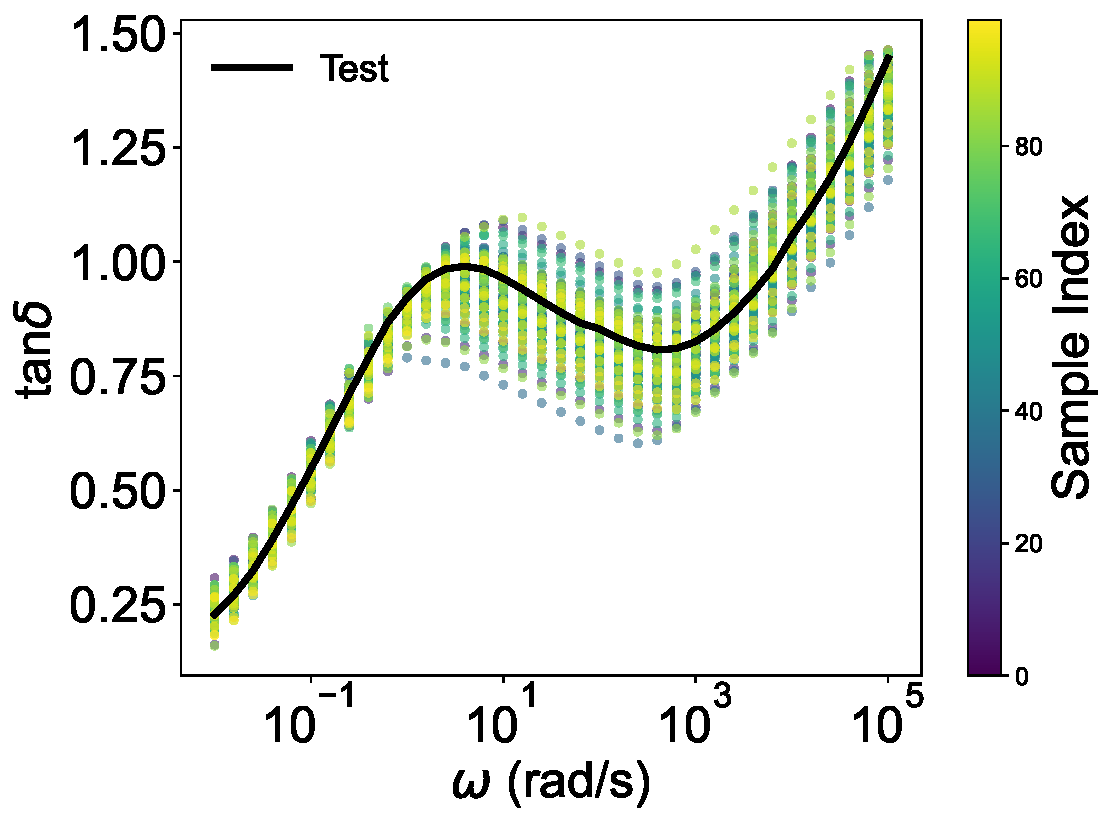
\includegraphics[width=0.8\textwidth]{Fig/prediction_results.pdf}
  \FigureBicaption{\label{cvae2pinn}100组CVAE生成的多模态解输入PINN模型后的预测值曲线}{Prediction curves of 100 multimodal solutions generated by CVAE after input into PINN model}
\end{figure}
从实验验证的角度考量,最理想的分析方法应该是按照生成的组分配比分别制备材料样品,通过DMA频率扫描实验测试其损耗角正切,并与目标曲线进行对比。然而,考虑到实验成本和时间效率,这种方法在实际操作中往往难以实现。为了在保证验证可靠性的同时提高效率,本节采用了一种替代方案:将CVAE模型生成的100组组分特征输入到已训练好的PINN模型中,通过PINN的预测结果来评估CVAE生成结果的质量。这种方法虽不能完全替代实验验证,但能在计算效率和验证可靠性之间取得较好的平衡。

图\ref{cvae2pinn}展示了这100组特征输入PINN后得到的频率-损耗角正切曲线,其中Test线代表原始真实特征对应的预测曲线。从图中可以观察到,这100组预测特征绘制的曲线形成了一个连续的曲线带,具有以下特点:首先,曲线带的整体趋势与Test线高度一致,表明生成的组分特征能够准确捕捉材料的主要流变学特性;其次,Test线位于曲线带的中心区域,说明生成结果的分布合理且具有代表性;最后,曲线带的宽度随频率变化呈现不均匀特征,这反映了在不同频率区间,组分配比对材料性能的影响程度各异。这种曲线带的分布特征有力地验证了CVAE模型在材料组分反演任务中的有效性和可靠性。

综上所述,通过PINN-CVAE联合建模方法的验证,我们不仅证实了CVAE在反向材料设计中的应用潜力,也验证了这种多模态解的实用价值。这种方法为高分子材料的智能设计提供了一种更为全面和灵活的解决方案,既保证了预测结果的物理合理性,又充分考虑了材料设计中固有的多解性特征。



% 本章小结 总结与展望
\section{本章小结}
本章主要围绕“高分子流变学的物理增强与逆向设计”这一主题,探索了PINN与CVAE两类深度学习模型在高分子流变学正向建模及组分反向设计中的应用。本章首先提出了PINN-CVAE联合建模的框架,构建了一个涵盖正向预测与反向设计的闭环系统,为高分子材料智能设计提供了全新思路。在这一框架下,PINN负责从组分特征到流变学性质的正向映射,而CVAE则实现从目标流变学性质到可能组分配比的反向生成,两者协同工作形成优化迭代系统。

在PINN正向建模部分,本章对比了传统DNN模型与基于物理先验约束的PINN模型在处理高维数据与复杂特征时的性能差异。PINN建模中采用了自适应权重机制,首先对PBA流体和单PBA注入制备的PFGs流体进行建模,结果表明PINN相比DNN具有更好的泛化预测效果。实验结果显示,普通PINN模型在一定程度上能够提高预测精度,但其泛化能力在特征数量较多且分布稀疏场景时表现一般,具体为在预测多组分PBA注入制备的PFGs流体时,模型预测效果较差。为此,本章进一步提出了两种特征融合改进方案——PINN-HP和PINN-AFF,通过预设和学习输入特征之间的物理关联,有效地改善了模型对各类复杂非线性关系的捕捉能力,从而解决特征稀疏的问题。从R$^2$、MAE、MAPE多项评价指标来看,PINN-AFF模型在预测准确性和稳定性上均明显优于传统DNN和普通PINN模型,尽管其训练时间略长,但整体优势十分明显,这为流变学数据的高精度预测提供了新思路。

在CVAE反向设计部分,本章深入探讨了利用CVAE模型进行材料组分反演的可行性。该部分工作主要通过将目标流变学参数(如$\omega$、$\mathrm{G^{\prime}}$、$\mathrm{G^{\prime\prime}}$和tan$\delta$)作为输入,生成多模态解,并对生成数据的残差分布、核密度及异常点进行了详细分析。结果表明,无论是分子量参数(Mn)还是组分含量参数($\phi$),生成数据均基本呈现正态分布特征,且随着参数数值的增大,预测误差逐步减小,MAPE指标均控制在较低水平,验证了模型在反向预测材料配方比例方面的高精度和鲁棒性。这一研究内容解决了传统回归方法单一输出的问题,而且为基于数据驱动的材料设计提供了具有多解性的参考方案,在真实的实验应用中可以使用这些多模态解来辅助调整实验设计,从而提高实验效率。

在PINN-CVAE联合建模验证中,本章通过将CVAE生成的100组组分特征输入已训练好的PINN模型,获得了这些组分对应的频率-损耗角正切曲线,形成了一个围绕真实曲线的连续曲线带。这种曲线带分布特征有力地验证了CVAE模型在材料组分反演任务中的有效性和可靠性,同时也体现了PINN-CVAE联合框架的实用价值。该联合框架既保证了预测的物理合理性,又提供了材料设计的多样化方案,为高分子材料的智能设计提供了完整解决方案。

此外,本章还对各模型在训练时间和资源消耗上的表现进行了比较和分析,指出尽管理论上PINN类模型由于引入了物理约束及复杂特征融合模块而导致训练时间较长,但其在捕捉复杂物理特性和有效泛化方面的优势足以弥补这一不足。同时,通过对比分析,可以发现深度学习模型在处理小数值参数时仍存在归一化误差,未来可通过调整量纲转换和数据预处理进一步优化模型效果。

综合来看,本章通过PINN-CVAE联合建模方法,系统性地解决了高分子流变学的正向预测与反向设计问题。PINN模型结合物理约束和特征融合机制,有效提高了流变学数据预测的准确性和泛化能力;CVAE模型则实现了从目标性能到多种可能配方的反向映射,为材料设计提供了多样化选择。两个模型相互配合,形成了一个自适应增强的流变学机器学习系统:CVAE生成的组分方案可通过PINN快速评估筛选,实验验证结果又可作为新数据反馈给模型进行训练,实现了从“正向预测-反向设计-实验验证-模型优化”的闭环迭代。这种结合物理信息与深度学习的联合建模方法,为高分子材料的智能设计和流变特性精准控制提供了新型数据驱动策略,具有重要的理论意义和应用前景。
